\section{Licensing lifecycle and migration evidence}\label{sec:C22:lifecycle}
Implementation visibility, artifact license, hosted-service terms, and operational inspectability are separate properties. A public repository can contain a client while the service remains proprietary. A source-visible license can restrict deployment or redistribution. A permissive core license may coexist with separately licensed connectors or enterprise features. The defensible statement identifies the inspected artifact and its license file at a revision; it does not attach an unqualified open-source label to an entire product family.

The inspected repository notices illustrate why this granularity matters. Mastra distinguishes its Apache-2.0 core from enterprise-licensed directories; n8n identifies Sustainable Use and Enterprise licenses; Dify identifies an Apache-2.0-derived license with additional conditions~\cite{executionproduct019,executionproduct057,executionproduct066}. These notices establish artifact-specific terms, not a universal compatibility judgment between deployments. DeepSeek Harness explicitly declares developer-preview status and anticipated compatibility-breaking changes~\cite{executionproduct035}. An active commit stream therefore does not establish a stable serialized-state or plugin ABI.

Lifecycle changes can invalidate comparisons even when names remain familiar. The inspected Llama Stack link resolves into the OGX lineage, and the Llama workflow link resolves to a broader agents repository. The Strands source link resolves to a harness SDK resource. These redirects are evidence of naming and packaging changes, not proof of complete backward compatibility. An application relying on old imports, storage schemas, or tool names needs a migration test rather than a renamed bibliography entry.

Historical products should be preserved where they explain architectural evolution, but they should not be described as active recommendations without current evidence. Archive status, maintenance activity, security-fix policy, and availability are distinct. A repository can remain readable after service termination; a commercial service can remain available while a legacy SDK is deprecated. The operating consequence is to maintain a dependency inventory with replacement and rollback plans, particularly for long-lived memory formats.

A migration experiment starts from a saved run and its authoritative state. Restore under the target release, validate schemas, rebuild indexes when required, and replay deterministic fixtures before permitting new model decisions. Compare tool availability, parser behavior, serialization, and cancellation. A test that merely imports the new package misses the semantics most likely to affect agent behavior. If the provider does not expose the necessary version controls, report that reproducibility limitation explicitly.

For a deterministic fixture, write $F_\nu:\mathcal S_\nu\times\mathcal U\to\mathcal S_\nu$ for a release's state transition and $O_\nu:\mathcal S_\nu\times\mathcal U\to\mathcal E$ for its observable event output. Let $m:\mathcal D\subseteq\mathcal S_\nu\to\mathcal S_{\nu'}$ be a partial migration with the same fixture inputs $\mathcal U$. On a transition-closed migration domain, require
\begin{align}
 m(F_\nu(s,u))&=F_{\nu'}(m(s),u),\\
 O_\nu(s,u)&=O_{\nu'}(m(s),u).
 \label{eq:C22:migration_commutes}
\end{align}
If both identities hold for every admitted $(s,u)$, induction on the finite input sequence gives identical fixture event traces and corresponding states after every step. This is a contract-preservation criterion, not a claim that all migrations satisfy it. The event space must include relevant tool intents, validation failures and recorded receipts; comparing only final chat strings discards precisely the events that can change effects. Real remote effects still require the service contract of Chapter~\ref{ch:C20}. A migration may legitimately reject an unsupported saved state; silently coercing it into another agent's state violates the criterion. A finite test suite provides evidence on its reached states, not proof of the universal identities. Stochastic model transitions require distributional comparison or fixed recorded outputs, rather than assuming identical samples.

Ownership and acquisition claims are excluded from technical inference unless primary evidence establishes them and they matter to the system boundary. Even a verified corporate change does not imply that products share code, data, or runtime guarantees. The analysis follows inspectable mechanisms and contracts. This avoids turning a provider map into an unsupported architectural map.


\subsection{Release-specific evidence at the October cutoff}
The official release records rechecked on 29 October identify LangGraph 1.2.18 on 26 October 2026, OpenAI Agents Python SDK 0.24.0 on 15 October, Google ADK 2.13.0 published on 23 October with release-note heading dated 22 October, and PydanticAI 2.63.0 on 28 October\cite{executionrelease01,executionrelease02,executionrelease03,executionrelease04}. These identifiers delimit the evidence; a current main branch can contain later or unreleased changes. Microsoft's repository has distinct .NET 1.26.0 and Python 1.23.0 releases, dated 23 and 22 October respectively, rather than one universal cross-language release\cite{executionrelease05,cumb2026mafpython}. CrewAI's inspected release was 1.15.32, while smolagents' latest returned release was 1.26.0 from May\cite{executionrelease07,executionrelease06}. Release recency alone is not a quality metric.

Several changes directly affect the consistency arguments in this book. LangGraph's notes change the default frequency of full delta snapshots from one thousand updates to one hundred, trading additional storage for faster reads on long threads. This is a concrete checkpoint-layout change, not evidence of better semantic memory. The Agents SDK notes defer automatic compaction during pending approvals, replace Redis compaction history atomically, and preserve completed tool outputs when a sibling fails. Those fixes identify distinct state boundaries: approval evidence, history replacement and partial parallel completion. They motivate targeted regression fixtures rather than a general claim that all consistency problems are solved\cite{executionrelease01,executionrelease02}.

ADK's release notes mark MongoDB session and memory services experimental even while promoting other features to stable status. They also change the default telemetry schema. Consequently, neither maturity nor trace compatibility should be assigned at whole-framework granularity. An analytics pipeline that assumes an older span layout can silently lose attribution after an otherwise successful upgrade. PydanticAI's notes change the default of its \texttt{CodeMode} dynamic catalog so newly revealed tools append rather than rewrite cached prompts. That is a component-specific context-construction choice whose effect depends on tool-discovery workload and cache behavior; it is not a universal change to every tool path or a measured application-level speedup\cite{executionrelease03,executionrelease04}.


Figure~\ref{fig:C22:overview} isolates the mechanism and its stated information boundaries.
\begin{figure}[!htbp]
\centering
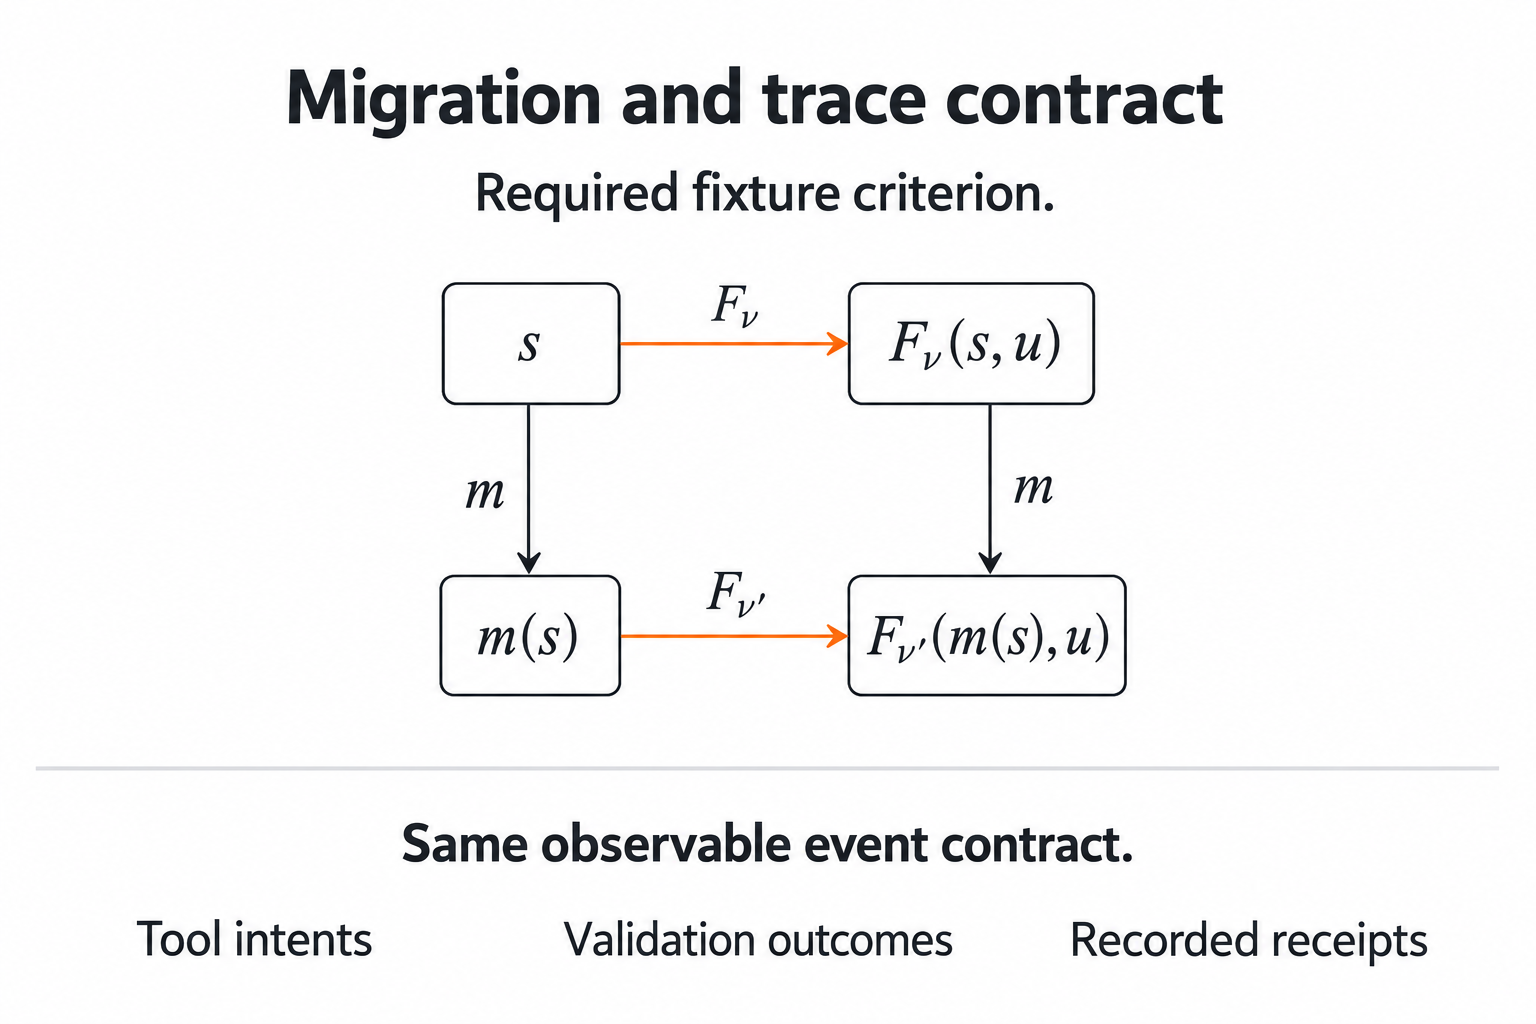
\includegraphics[width=\linewidth]{book/figures/assets/F22review.png}
\caption{A deterministic migration criterion compares the two paths through corresponding fixture states. On an admitted transition-closed domain, migration must commute with the state transition and preserve the declared observable events. Finite fixtures test reached states; they do not prove the universal identities or establish remote-effect uniqueness.}
\label{fig:C22:overview}
\end{figure}
